%%%%%%%%%%%%%%%%%%%%%%%%%%%%%%%%%%%%%%%%%
%
% CMPT 435
% Lab Zero
%
%%%%%%%%%%%%%%%%%%%%%%%%%%%%%%%%%%%%%%%%%

\documentclass[letterpaper, 10pt]{article} 

\usepackage[english]{babel} % English language/hyphenation
\usepackage{graphicx}
\usepackage[lined,linesnumbered,commentsnumbered]{algorithm2e}
\usepackage{listings}
\usepackage{xcolor}
\usepackage{float}
\usepackage{fancyhdr} % Custom headers and footers
\pagestyle{fancyplain} % Makes all pages in the document conform to the custom headers and footers
\usepackage{lastpage}
\usepackage{url}
\usepackage{multirow}

\definecolor{codegreen}{rgb}{0,0.6,0}
\definecolor{codegray}{rgb}{0.5,0.5,0.5}
\definecolor{codepurple}{rgb}{0.58,0,0.82}
\definecolor{backcolour}{rgb}{0.95,0.95,0.92}

\lstset{       
    language=c++,
    backgroundcolor=\color{backcolour},   
    commentstyle=\color{codegreen},
    keywordstyle=\color{magenta},
    numberstyle=\tiny\color{codegray},
    stringstyle=\color{codepurple},
    basicstyle=\ttfamily\footnotesize,
    breakatwhitespace=false,         
    breaklines=true,                 
    captionpos=b,                    
    keepspaces=true,                 
    numbers=left,                    
    numbersep=5pt,                  
    showspaces=false,                
    showstringspaces=false,
    showtabs=false,                  
    tabsize=2                    
}

\fancyhead{} % No page header - if you want one, create it in the same way as the footers below
\fancyfoot[L]{} % Empty left footer
\fancyfoot[C]{page \thepage\ of \pageref{LastPage}} % Page numbering for center footer
\fancyfoot[R]{}

\renewcommand{\headrulewidth}{0pt} % Remove header underlines
\renewcommand{\footrulewidth}{0pt} % Remove footer underlines
\setlength{\headheight}{0pt} % Customize the height of the header

%----------------------------------------------------------------------------------------
%	TITLE SECTION
%----------------------------------------------------------------------------------------

\newcommand{\horrule}[1]{\rule{\linewidth}{#1}} % Create horizontal rule command with 1 argument of height

\title{	
   \normalfont \normalsize 
   \textsc{CMPT 435 - Fall 2024 - Dr. Labouseur} \\[10pt] % Header stuff.
   \horrule{0.5pt} \\[0.25cm] 	% Top horizontal rule
   \huge Assignment One -- Data Structures \\ and Sorting \\     	    % Assignment title
   \horrule{0.5pt} \\[0.25cm] 	% Bottom horizontal rule
}

\author{Tyler DeLorey \\ \normalsize tyler.delorey1@marist.edu}

\date{\normalsize\ October 4th, 2024}

\begin{document}
 
\maketitle % Print the title

%----------------------------------------------------------------------------------------
%   CONTENT SECTION
%----------------------------------------------------------------------------------------

% Reset figure numbering to include section number
\renewcommand{\thefigure}{\thesection.\arabic{figure}}

\vspace{-5em}
\tableofcontents

\section{C++ Basics}
\subsection{Introduction}

\noindent
I used C++ to complete this assignment. Before I start explaining about stacks and queues, palindromes, and each sort, I just want to justify some of the things I did that are C++ specific, like creating the header files, using vectors, and how I input the magicitems.txt file. This hopefully will explain some things that in my code that may seem odd, but are actually reasonable.

\subsection{Header Files}
\noindent
The first thing I want to talk about are how I used header files. Header files in C++ (.h files) typically contain just function declarations and class definitions, while the corresponding .cpp file contains the implementations of those functions and classes. In my case, however, because most of the code is short and simple, I just put the implementations in the .h file and got rid of the corresponding .cpp files to avoid confusion. This is why there is only one .cpp file for this assignment (main.cpp). The five header files for this assignment are Node.h, Stack.h, Queue.h, isPalindrome.h, and Sorts.h. I will be explaining each in-depth in the future sections. 

\subsection{Makefile}
\noindent
In order to make compiling my code easier, I created a Makefile. By simply running the command "make" (assuming the g++ and make commands are installed on your system), the code will compile automatically and all output will return in the terminal. I also tried to make it compatible for Windows and Linux users, which took me hours to complete. This was difficult mostly due to the "make clean" command I implemented, which removes the unnecessary files created after the "make" command was run. Because these files differ between Windows and Linux, the command would have to run differently depending on the operating system you are using. Figure 1.1 below shows how I implemented Makefile for this assignment (sorry if syntax highlighting looks bad, it's configured for C++ code).

\begin{figure}[H]
  \centering
  \lstinputlisting[firstline=1, lastline=11]{Makefile} % First part of the Makefile
  \label{fig:figure1.1_part1}
\end{figure}

\begin{figure}[H]
  \centering
  \lstinputlisting[firstline=12, firstnumber=12]{Makefile} % Second part of the Makefile
  \caption{Makefile}
  \label{fig:figure1.1_part2}
\end{figure}
\noindent
The Makefile compiles the .cpp files into .o files with the header dependencies, then it runs the executable code. In order for the "make clean" command to work, I have to use the "del" command for Windows and "rm" command for Linux. I also have the specify the correct executable to remove. The executable differs depending on what operating system it is run on. On Windows, the executable is main.exe while it is just main on Linux systems. 

\subsection{Reading from File}
\noindent
I know this information isn't that at all exciting or necessary (sorry for this), but I had to learn how to implement C++ file IO in order to use the magicitems.txt file in my program. Figure 1.2 below shows how I read from the file. 
\begin{figure}[H]
  \centering
  \lstinputlisting[firstline=1, lastline=7]{main.cpp} 
  \label{fig:figure1.2_part1}
\end{figure}

\begin{figure}[H]
  \centering
  \lstinputlisting[firstline=8, firstnumber=8, lastline=39]{main.cpp} 
  \caption{File Reading (main.cpp)}
  \label{fig:figure1.2_part2}
\end{figure}
\noindent
On Line 2, I included the file stream library, which provided classes for reading and writing files or data streams. I used the structure ifstream which can read from files on Line 22. I used the structure to open the file (Line 25). After making sure the file is opened and valid (Lines 26-30), I had to read each line from the file to put into an array (Lines 33-36). I used C++ vectors in order to store all of the data from the file. 

\subsection{Vectors}
\noindent
Vectors in C++ are like ArrayLists in Java. It is a dynamic array that can grow or shrink in size. To use, I had to include the vector library (as shown in Line 3 of Figure 1.2). Then I named the specified it to be a string vector (a vector that holds string) and named it magicItems (Line 13). In order to push items to the vector, I used the push\_back function and pushed each line from the file I read (Line 35). After these steps, it mostly functions as any other array. For example, it uses bracket notation, indices, and it is hard to tell apart from a normal array. If I refer to magicItems as an array in this documentation or comments in the code, I mean it's a vector. I like the use the word array since it's something I'm more familiar with.

\section{Stacks and Queues}
\setcounter{figure}{0} % Reset figure counter

\subsection{Node Class}
\noindent
Before I start explaining how I implemented my own Stacks and Queues in my program, I need to explain my Node class. 
\begin{figure}[H]
  \centering
  \lstinputlisting[]{Node.h} 
  \caption{The Node Class (Node.h)}
  \label{fig:figure2.1}
\end{figure}
\noindent
The Node class contains data and a next pointer, as defined on Lines 14 and 17 respectively. The data variable stores a single character for each Node, while the next pointer points to the next Node. When the Node function is called with a parameter value, the data gets set to that value, and the next pointer initially gets set as null (Lines 20-24). These pointers are adjusted when working with the Stack and Queue classes. With the Node class setup, a linked list can be created, where a Node has a pointer to another Node, and that Node has a pointer to another, and etc. This is how the Stacks and Queues are implemented. 

\subsection{Stack Class}
\noindent
The Stack class and its functions are all declared and initialized in my Stack.h file. My Stack has three functions associated with it: push, pop, and isEmpty. 
\begin{figure}[H]
  \centering
  \lstinputlisting[firstline=1, lastline=50]{Stack.h} 
  \label{fig:figure2.2_part1}
\end{figure}

\begin{figure}[H]
  \centering
  \lstinputlisting[firstline=51, firstnumber=51]{Stack.h} 
  \caption{The Stack Class (Stack.h)}
  \label{fig:figure2.2_part2}
\end{figure}
\noindent
The Stack I implemented is essentially a linked list of Nodes with a pointer named "top" that points to the Node on top of the stack. The three main functions associated with this class have the time complexity of O(1), meaning they run in constant time. 
\noindent
\begin{itemize}
  \item Line 25: The "push(char item)" function creates a new Node with the provided parameter as its data. The new Node's next pointer is set to the current top of the Stack (or nullptr if the Stack was previously empty). The new Node then becomes the new top of the stack.
  \item Line 34: The "pop()" function removes the top Node from the Stack and returns its data if it isn't empty. It deletes that Node from memory and sets the new top to the Node referenced by the previous top's next pointer.
  \item Line 52: The "isEmpty()" function checks whether the Stack is empty by seeing if the top pointer references a valid Node.
\end{itemize} 
\noindent
In order to avoid memory leaks, I had to also implement a deconstructor for the Stack (Line 15), which pops all Nodes from the Stack when the Stack object is destroyed. The deconstructor ensures that all Nodes are popped and deallocated from memory.  

\subsection{Queue Class}
The Queue has a ton of similarities to the Stack class, so sorry if this information seems very repetitive. The Queue class and its functions are all declared and initialized in my Queue.h file. My Queue has three functions associated with it: enqueue, dequeue, and isEmpty. 
\begin{figure}[H]
  \centering
  \lstinputlisting[firstline=1, lastline=8]{Queue.h} 
  \label{fig:figure2.3_part1}
\end{figure}

\begin{figure}[H]
  \centering
  \lstinputlisting[firstline=9, firstnumber=9, lastline=60]{Queue.h} 
  \label{fig:figure2.3_part2}
\end{figure}

\begin{figure}[H]
  \centering
  \lstinputlisting[firstline=61, firstnumber=61]{Queue.h} 
  \caption{The Queue Class (Queue.h)}
  \label{fig:figure2.3_part3}
\end{figure}
\noindent
Like with the Stack class, the three main functions associated with Queue have the time complexity of O(1), meaning they run in constant time. Unlike the Stack however, I implemented the Queue class using two pointers to keep track of the Nodes in the linked list instead of just one. There is a head pointer which keeps track of the head of the list, and there is a tail pointer which keeps track of the tail of the list.
\noindent
\begin{itemize}
  \item Line 26: The "enqueue(char item)" function creates a new Node with the provided parameter as its data. If the Queue is not empty, the current tail's next pointer is set to the new Node, and the new Node becomes the new tail. If the queue is empty, the new Node becomes both the head and tail of the queue.
  \newline
  The reason why I included the tail pointer was to make the enqueue function O(1) instead of O(n). If I only had a pointer to the head, I would have to traverse the entire linked list to get to the end of the list, which would be an O(n) operation. 
  \item Line 44: The "dequeue()" function removes the head Node from the Queue and returns its data if it isn't empty. It deletes that Node from memory and sets the new head to the Node referenced by the previous head's next pointer.
  \item Line 62: The isEmpty() function checks whether the Queue is empty by seeing if the head pointer references a valid Node.
\end{itemize} 
\noindent
Like with the Stack class, I had to implement a deconstructor for the Queue (Line 17) to avoid memory leaks, which dequeues all Nodes from the Queue when the Queue object is destroyed. The deconstructor ensures that all Nodes are dequeued and deallocated from memory.  

\section{Palindromes}
\setcounter{figure}{0} % Reset figure counter
\subsection{Introduction}
\noindent
The established Stack and Queue classes are used in order to check if words are palindromes or not. Figure 3.1 below shows partly how this is done.
\begin{figure}[H]
  \centering
  \lstinputlisting[firstline=41, firstnumber=41, lastline=53]{main.cpp}
  \caption{Palindrome Checking (main.cpp)}
  \label{fig:figure3.1}
\end{figure}
\noindent
To check if each word in the magicItems array is a palindrome, the whole list has to be looped through (Line 43). Each word is passed through a "isPalindrome" function to check if it a palindrome (this function will be further discussed). If the function returns true, the word will be displayed and the palindrome counter will increase (Lines 49 and 50). After the loop completes, the program displays the number of palindromes on Line 53. 

\subsection{isPalindrome: Pushing and Enqueuing Letters}
\noindent
The isPalindrome function is located in the isPalindrome.h header file. Below is the first half of the function, which focuses on pushing letters onto the Stack and enqueuing letters to the Queue.
\begin{figure}[H]
  \centering
  \lstinputlisting[lastline=18]{isPalindrome.h}
  \label{fig:figure3.2-part1}
\end{figure}

\begin{figure}[H]
  \centering
  \lstinputlisting[firstline=19, firstnumber=19, lastline=36]{isPalindrome.h}
  \caption{Pushing and Enqueuing Letters (isPalindrome.h)}
  \label{fig:figure3.2-part2}
\end{figure}

\begin{figure}[H] 
    \centering 
    \fbox{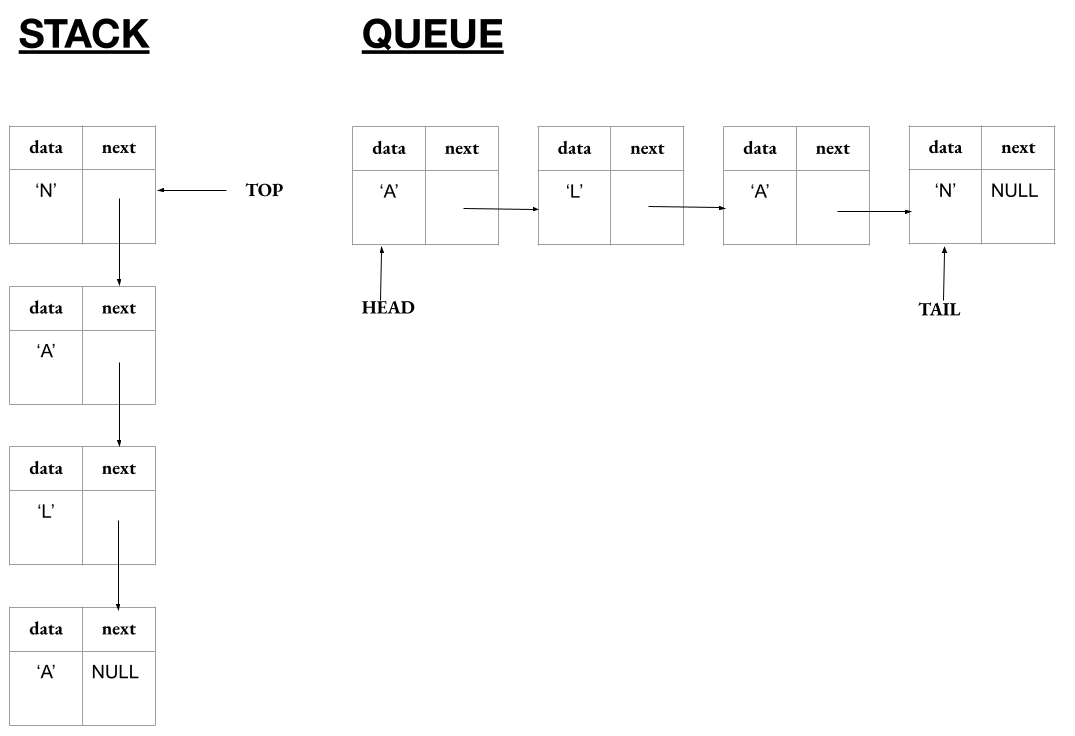
\includegraphics[width=0.98\textwidth]{./imgs/StackandQueueEX.png}}
    \caption{Stack and Queue Example for isPalindrome.h}
    \label{fig:figure3-3}
\end{figure}
\noindent
Before pushing and enqueuing letters into the Stack and Queue, the classes need to be initialized. I created a Stack and a Queue named myStack and myQueue for the word passed into the function on Lines 13 and 14. The for-loop on Line 26 iterates through each letter in the word. In this program, palindromes ignore capitalization and spaces, so the program automatically converts each character to uppercase (Line 28) and checks if the character is not a space (Line 30). If the character is not a space, it is pushed onto the Stack and enqueued in the Queue (Lines 32 and 33). Each letter is stored as the data in a new Node. Once the for-loop is complete, the Stack and Queue will be full of Nodes representing the uppercase letters. The program will also have the size of the Stack and Queue, tracked by the "sizeWithoutSpaces" variable that increments each time a push and enqueue occurs (Line 34). Figure 3.3 above is an example of what the Stack and Queue would look like at the step if the parameter passed into the function was the word 'Alan'.

\subsection{isPalindrome: Popping and Dequeuing Letters}
\noindent
After adding the valid letters as Nodes in the Stack and Queue, it is reasonable to pop and dequeue each letter one at a time and compare them. A palindrome is spelled the same forwards as it is backwards. Since the Stack is essentially reversing the word, the letter popped from the Stack should always match the letter dequeued from the Queue if the word is a palindrome.
\begin{figure}[H]
  \centering
  \lstinputlisting[firstline=38, firstnumber=38]{isPalindrome.h}
  \caption{Popping and Dequeuing Letters (isPalindrome.h)}
  \label{fig:figure3.4}
\end{figure}
\noindent
The loop on Line 39 iterates for each letter there is in the Stack and the Queue. The letter at the top of the Stack is popped and the letter at the head of the Queue is dequeued on Lines 41 and 42. Like stated earlier, if these letters don't match, the word is not a palindrome and the loop is broken out of (Lines 44-49) to return false. If the letters match, the word could possibly be a palindrome, but it has to keep iterating through the entire loop. If the letters always match throughout the entire loop, the function returns true, meaning that the word was indeed a palindrome. Looking back at Figure 3.3, the word 'Alan' is obviously not a palindrome because 'N' (popped value from Stack) and 'A' (dequeued value from Queue) are not equal.
For the case of magicitems.txt, out of the 666 "words" in the array, only 15 of them were palindromes. They are displayed in Table 1.
\begin{table}[H]
    \centering
    \begin{tabular}{|l|}
        \hline
        \textbf{Palindromes} \\ \hline
        Boccob \\ 
        Seuss Igniting Issues \\ 
        UFO tofu \\ 
        Ebuc Cube \\ 
        Aibohphobia \\ 
        Taco cat \\ 
        Was It A Rat I Saw \\ 
        Olah Halo \\ 
        CD case divides ACDC \\ 
        Dacad \\ 
        Dior Droid \\ 
        Robot Tobor \\ 
        Narc in a panic ran \\ 
        radar \\ 
        Golf flog \\ \hline
    \end{tabular}
    \caption{Palindromes in the magicitems.txt file}
    \label{tab:tab1}
\end{table}

\section{Sorting}
\setcounter{figure}{0} % Reset figure counter
\subsection{Introduction}
\noindent
Now that the palindrome program is all figured out, it is time to explain the sorts. This assignment tasked us to do four different sorts: Selection Sort, Insertion Sort, Merge Sort, and Quick Sort. The sorts are implemented in the Sorts.h file and are run on the magicItems array. The figure below shows the sort functions being called in main, with the number of comparisons being displayed for each sort.
\begin{figure}[H]
  \centering
  \lstinputlisting[firstline=55, firstnumber=55, lastline=61]{main.cpp}
  \label{fig:figure4.1-part1}
\end{figure}

\begin{figure}[H]
  \centering
  \lstinputlisting[firstline=62, firstnumber=62, lastline=83]{main.cpp}
  \caption{Calling Sort Functions (main.cpp)}
  \label{fig:figure4.1-part2}
\end{figure}
\noindent
Before each sort is called, the array is passed through a shuffle function which randomly rearranges the contents in the array. Then the array is passed through the sort functions, which returns the number of comparisons the sort had to make. Then, the comparison count is displayed in the terminal.

\noindent
QUICK NOTE: The sorts work in ASCII-order, meaning all of the lowercase strings will be after the uppercase ones. All sorts are case sensitive. In the magicitems.txt file, there are only about nine strings that are lowercase, so the results shouldn't look super jarring.

\subsection{Shuffle Function}
\noindent
Before calling each sort, the shuffle function is called, which shuffles the entire array. I did this by implementing a shuffle routine based on the Knuth, or Fisher-Yates, shuffle.
\begin{figure}[H]
  \centering
  \lstinputlisting[lastline=7]{Sorts.h}
  \label{fig:figure4.2-part1}
\end{figure}

\begin{figure}[H]
  \centering
  \lstinputlisting[firstline=8, firstnumber=8, lastline=34]{Sorts.h}
  \caption{Shuffle Function (Sorts.h)}
  \label{fig:figure4.2-part2}
\end{figure}
\noindent
The shuffle function iterates through the entire array from the end to the beginning (Line 19). In each iteration, a random index from non-shuffled part of the array is chosen (Lines 22-26), and the item at that random index is swapped with the item at the current index (Lines 29-31). This makes it so the entire array is shuffled when the loop completes.

\noindent
In order to compute the random index, instead of using the rand() function, I included the random library (Line 6). I realized that the rand() function isn't all that random because each time I compiled the code I would always get the same "random" results. With the random library, using the structures provided, it makes the random index TRULY random.

\subsection{Selection Sort}
\noindent
Selection sort works by finding the smallest value in the unsorted section of the array, and swapping it with the first element of that section. 
\begin{figure}[H]
  \centering
  \lstinputlisting[firstline=36, firstnumber=36, lastline=39]{Sorts.h}
  \label{fig:figure4.3-part1}
\end{figure}

\begin{figure}[H]
  \centering
  \lstinputlisting[firstline=40, firstnumber=40, lastline=70]{Sorts.h}
  \caption{Selection Sort (Sorts.h)}
  \label{fig:figure4.3-part2}
\end{figure}

\vspace{-0.5em}
\noindent
The outer loop (Line 45) iterates through the entire array, excluding the last index, with the variable i tracking the current position to be sorted. The inner loop (Line 50) iterates through the remaining unsorted part of the array to find the minimum value (Line 53). The index of this minimum value is stored in the minIndex variable (Line 55). After the inner loop completes, if the minimum value is not already at position i, the element at minIndex is swapped with the element at i (Lines 61-66), placing the smallest element in its correct position. Here is a sort result of running Selection Sort five times:
\begin{table}[H]
\centering
\begin{tabular}{|c|c|c|}
\hline
\textbf{Input Size (n)} & \textbf{Number of Comparisons} & \textbf{Time Complexity} \\
\hline
\multirow{5}{*}{666} & 221,445 & \\
                     & 221,445 & \\
                     & 221,445 & $O(n^2)$ \\
                     & 221,445 & \\
                     & 221,445 & \\
\hline
\end{tabular}
\caption{Selection Sort Results (Average Num of Comparisons: 221,445)}
\end{table}

\noindent
The time complexity of Selection Sort is $O(n^2)$ because there are nested loops. The outer loop iterates through the array (n - 1) times, and the inner loop iterates through the array (n - i - 1) times, meaning as the variable "i" increases, the inner loop iterates through less and less because more and more of the array is being sorted. When multiplying (n - 1) and (n - i - 1), and ignoring constant factors and only looking at the most dominant function of n, it results to $n^2$. Selection Sort will always have the same number of comparisons no matter how the list is sorted beforehand. The inner loop first makes n - 1 comparisons, then n - 2, then n - 3, all the way down to 1. This can all be summed up to $(n-1)(n-1+1)/2$, or $n(n-1)/2$, and when plugging in the input size of the magicItems array (666) for n, it results to 221445. 

\subsection{Insertion Sort}
\noindent
Insertion sort works by building a sorted section of the array one element at a time, repeatedly picking the next element and inserting it into its correct position relative to the already sorted elements.
\begin{figure}[H]
  \centering
  \lstinputlisting[firstline=72, firstnumber=72, lastline=97]{Sorts.h}
  \label{fig:figure4.4-part1}
\end{figure}

\begin{figure}[H]
  \centering
  \lstinputlisting[firstline=98, firstnumber=98, lastline=103]{Sorts.h}
  \caption{Insertion Sort (Sorts.h)}
  \label{fig:figure4.4-part2}
\end{figure}

\noindent
The outer loop (Line 80) iterates through the entire array, excluding the first index (it's technically already sorted in an array of size 1), with the variable i tracking the current position to be sorted. The inner loop (Line 89) helps find the correct index to place the current "key" value. It achieves this by shifting rest of the element to the right if the position is not correct (Lines 92-93). Once the inner loop is completed, that means it found the correct position, and the key value is inserted there (Line 99). 
Here is a sort result of running Insertion Sort five times:
\begin{table}[H]
\centering
\begin{tabular}{|c|c|c|}
\hline
\textbf{Input Size (n)} & \textbf{Number of Comparisons} & \textbf{Time Complexity} \\
\hline
\multirow{5}{*}{666} & 120,103 & \\
                     & 108,403 & \\
                     & 109,636 & $O(n^2)$ \\
                     & 112,684 & \\
                     & 108,552 & \\
\hline
\end{tabular}
\caption{Insertion Sort Results (Average Num of Comparisons: 111,876)}
\end{table}

\vspace{-0.5em}
\noindent
Like Selection Sort, the time complexity of Insertion Sort is $O(n^2)$ because there are nested loops. The outer loop iterates through the array (n - 1) times. Depending on where the correct position is for the key value, the inner loop can run up to i times in a worst case scenario. Since the variable i will eventually be n - 1, there is essentially an equation that will have n multiplied by n (in a worst case scenario), which results in $n^2$, and since that's all that is cared about (ignoring constant factors and it's the most dominant function of n), the time complexity of Insertion Sort is $O(n^2)$. Calculating the number of comparisons is quite difficult because unlike Selection Sort, the number of comparisons actually depend on the original order of the array. No matter what, the first loop is run (n - 1) times. On average, the inner loop would be ran (i / 2) times. The total comparisons can be defined as the summation $\sum_{i = 1}^{n-1} i$. Since this is essentially adding up the first n - 1 integers, this can be rewritten as $(n-1)(n-1+1)/2$, or $n(n-1)/2$. This is all multiplied by $1/2$ because on average, the key value is being compared with half of the previous elements (hence the i / 2). Multiplying these numbers results in approximately $n^2/4$. Plugging in 666 for n results in 110,889. This is approximately the average number of comparisons Insertion Sort performs with an input array of size 666. Selection Sort and Insertion Sort have the same big-Oh time complexity, but Insertion Sort does half the amount of comparisons that Selection Sort does.

\subsection{Merge Sort}
\noindent
Merge Sort takes a different approach than Selection Sort and Insertion Sort. Merge Sort does a divide and conquer technique by recursively splitting the array into halves, and then merges the  halves back together, sorting them on the way, to produce a fully sorted array. I will first explain the divide step of Merge Sort.
\begin{figure}[H]
  \centering
  \lstinputlisting[firstline=160, firstnumber=160, lastline=189]{Sorts.h}
  \caption{mergeSort function (Sorts.h)}
  \label{fig:figure4.5}
\end{figure}
\noindent
The mergeSort function essentially gets the mid point to split the array into two halves (Line 179), and then recursively calls itself twice with parameters signifying that it's the left and right sides of the original array (Lines 182 and 183). The function will keep being called recursively until the array is of size 1. In this case, where the beginning index is greater than or equal to the ending index, it will terminate (Line 175). 
\vspace{1em}
This is the base case for the function. 

\noindent
Something interesting that I decided to do for this program was to not have any extra parameters in the original call of the function in main.cpp (Line 73 of Figure \ref{fig:figure4.1-part2} shows the program calling mergeSort(magicItems) with no other parameters). I wanted to do this to increase readability for the main function, instead of also including the begin and end index parameters in the function call, which would be 0 and n - 1 respectively. To do this, I had to use default parameters. A problem came with this because I couldn't set the default parameter for the variable "end" to myItems.size() - 1 because an error would occur stating that myItems may not appear in that context. I think the error occurs because myItems wouldn't be accessible whenever the function was declared because it isn't static. I came up with a workaround to this error. I set the "end" variable to INT\_min as a default parameter, and if that variable was equal to INT\_MIN, it would be changed to equal myItems.size() - 1 (Lines 168-171) because that's the last index of the whole array.
\vspace{1em}

\noindent
Now that I covered the dividing step of Merge Sort, next up the conquer step. I implemented this by creating a merge function (called on Line 186 of mergeSort).
\begin{figure}[H]
  \centering
  \lstinputlisting[firstline=105, firstnumber=105, lastline=136]{Sorts.h}
  \label{fig:figure4.6-part1}
\end{figure}
\begin{figure}[H]
  \centering
  \lstinputlisting[firstline=137, firstnumber=137, lastline=158]{Sorts.h}
  \caption{Merge Function (Sorts.h)}
  \label{fig:figure4.6-part2}
\end{figure}
\noindent
The merge function begins by initializes some variables that keep track of the current index for both the left and right portions of the array (Line 111). It also keeps track the size of each portion (Lines 112, 113) and adds them up to get the size of the merged array (Line 116). To actually merge the two portions successfully, there needs to be another array that holds the values temporary (Line 118). Because I'm using a temporary vector, this means that the sort is not in-place (I'm using more than a constant amount of space in order to complete the sort). After declaring the tempItems vector of size n, a loop iterates through each of these indexes to see what value should be put in what places (Line 121). The four cases are as follows:
\begin{itemize}
  \item Lines 126-130: If the right portion was completely ran through, then copy the remaining left portion items into the temporary vector. 
  \item Lines 132-135: If the left portion was completely ran through, then copy the remaining right half items into the temporary vector
  \item Lines 138-142: If the current element in the left portion is less than the current element in the right portion, then choose the element in the left portion to copy to the temporary vector
  \item Lines 144-148: If the current element in the right portion is less than the current element in the left portion, then choose the element in the right portion to copy to the temporary vector.
\end{itemize}
\noindent
After the loop is complete, the tempItems vector should be completely full of values that are sorted. However, these sorted values are no good if they aren't copied back over to the original vector (myItems). Lines 152-155 focus on copying the values from tempItems back over to myItems in the correct positions.
Here is a sort result of running Merge Sort five times:
\begin{table}[H]
\centering
\begin{tabular}{|c|c|c|}
\hline
\textbf{Input Size (n)} & \textbf{Number of Comparisons} & \textbf{Time Complexity} \\
\hline
\multirow{5}{*}{666} & 6,302 & \\
                     & 6,302 & \\
                     & 6,302 & $O(n * log(n))$ \\
                     & 6,302 & \\
                     & 6,302 & \\
\hline
\end{tabular}
\caption{Merge Sort Results (Average Num of Comparisons: 6,302)}
\end{table}

\noindent
Unlike Selection Sort and Insertion Sort, the time complexity of Merge Sort is $O(n * log(n))$. The reason why is it isn't $O(n^2)$ is because there aren't nested loops. Instead, there are recursive calls. The $n$ portion of $n * log(n)$ is because the merge function runs through the first loop $n$ times (can ignore the second loop at Line 152 because it also runs $n$ times, and $n + n = 2n$ is irrelevant because asymptotic running time ignores constant factors). The $log(n)$ comes from the recursive calls. Let's say there is an array of size 8. The amount of divides it would take to get the array to the size of one is 3 $(8 \rightarrow 4 \rightarrow 2 \rightarrow 1)$. The amount of divides it would take to get an array of size 32 to an array of size 1 is 5 $(32 \rightarrow 16 \rightarrow 8 \rightarrow 4 \rightarrow 2 \rightarrow 1)$. This is basically what $\log_2(n)$ is, where $\log_2(8) = 3$ and $\log_2(32) = 5$. Since asymptotic running time ignores constant factors, $log(n)$ is the time complexity of the dividing step, and $n$ is the time complexity of the conquering step, resulting in $O(n * log(n))$. Also, like Selection Sort, the amount of comparisons are always the same, no matter how the array was previously sorted before being passed into the functions. It is actually easier to count the number of comparisons with Merge Sort than it is with Selection Sort and Insertion Sort. It is just $n * \log_2(n)$. This is because Merge Sort can be written as the recurrence relation $T(n) = T(n/2) + T(n/2) + n$. The two $T(n/2)$ represent the dividing and the $n$ represents the conquering. Trying to solve this equation eventually results in $T(n * \log_2(n))$. Plugging in 666 for n results in approximately 6,247. This is very close to the number of comparisons I got in my program. Merge Sort is faster and does less comparisons then both Selection and Insertion Sort. However, Merge Sort is not an in-place sort, while Selection Sort and Insertion Sort are, because I used the tempItems vector to store some information in the merge function.

\vspace{3em}
\subsection{Quick Sort}
\noindent
Quick Sort takes a very similar approach compared to Merge Sort. Quick Sort also does a divide and conquer, but instead of doing it in two different steps, it does it at the same time. I will first explain the quickSort function before I get into the partition one.
\begin{figure}[H]
  \centering
  \lstinputlisting[firstline=230, firstnumber=230, lastline=271]{Sorts.h}
  \label{fig:figure4.7-part1}
\end{figure}

\begin{figure}[H]
  \centering
  \lstinputlisting[firstline=272, firstnumber=272]{Sorts.h}
  \caption{quickSort function (Sorts.h)}
  \label{fig:figure4.7-part2}
\end{figure}
\noindent
Quick Sort works by choosing a pivot value. The arrays are recursively divided (like Merge Sort) into two different sections split up by a value from the partition function (will be explained later). Conquering occurs by partitioning those two sections until the smallest sub-arrays are sorted. To choose a pivot value, I used three contenders to avoid getting the absolute worst case possible: when the pivot value is on either end of the array. This could result in $O(n^2)$ time complexity, which isn't wanted. The contenders are random indexes in the array (Lines 247-252). To not get the absolute worst pivot, I compared the three contenders and chose the one in the middle to be the pivot (Lines 255-267). After the pivot index is chosen, the partition function is called (Line 270), which returns the partition index that splits the array into two. To split the array, the quickSort function is recursively called with the two parts (excluding the partition index), kind of like how Merge Sort recursively called the two halves of that array.

\noindent
Lines 236-244 of the quickSort function are exactly the same as the mergeSort function, so the explanation of why the code looks the way it does is in the Merge Sort section. The initial end index of the array is myItems.size() - 1, and if the array is of size 1, then it terminates (Base Case). 

\noindent
Now that I explained the quickSort function, it is time to talk about the partition function.
\begin{figure}[H]
  \centering
  \lstinputlisting[firstline=191, firstnumber=191, lastline=198]{Sorts.h}
  \label{fig:figure4.8-part1}
\end{figure}

\begin{figure}[H]
  \centering
  \lstinputlisting[firstline=199, firstnumber=199, lastline=226]{Sorts.h}
  \caption{Partition function (Sorts.h)}
  \label{fig:figure4.8-part2}
\end{figure}

\noindent
The main goal of the partition function is to ensure that all elements less than the pivot are moved to the left side and all elements greater than the pivot are moved to the right side. The function starts of by declaring the variable "l" which indicates the current partition position (Line 197). It then swaps the pivot index value and the value at the end of the array, which essentially just moves the pivot value to the end (Lines 200-202). Then a loop runs for every index in that sub-array range (Line 204), where if the current element is less than the pivot value, it will swap the value at the current iterated index in the loop with the partition index value (Lines 209-218). This ensures that the smaller element is in the left side of the partition. After the loop is complete, the pivot and partition indexes are swapped to put the pivot in the correct position (Lines 221-223).

\noindent
Quick Note: the reason why the function returns a pair is because even though I need the partition index to actually make the sort work, I also need the comparison count. This is why the function return type is <int, int> (it's returning two separate values).

\vspace{1em}
\noindent
Here is a sort result of running Quick Sort five times:
\begin{table}[H]
\centering
\begin{tabular}{|c|c|c|}
\hline
\textbf{Input Size (n)} & \textbf{Number of Comparisons} & \textbf{Time Complexity} \\
\hline
\multirow{5}{*}{666} & 6,468 & \\
                     & 6,245 & \\
                     & 7,084 & $O(n * log(n))$ \\
                     & 6,541 & \\
                     & 6,329 & \\
\hline
\end{tabular}
\caption{Quick Sort Results (Average Num of Comparisons: 6,533)}
\end{table}

\noindent
Exactly like Merge Sort, the time complexity of Quick Sort is $O(n * log(n))$. There are recursive calls instead of nested loops. The $n$ portion of $n * log(n)$ is because the partition function runs through the loop approximately $n$ times. The $log(n)$ comes from the recursive calls in the quickSort function. Also, like Insertion Sort, but unlike Merge Sort and Selection Sort, the amount of comparisons are different each time the function gets called. This is because it depends on the pivot values chosen, which are random in this case. Because of this, it is very difficult to come up with an equation to help find the average number of comparisons Quick Sort does. But, according to the table above, the average number of comparisons were 6,533. This is approximately equal to $n * log(n)$ with n = 666 in this case, like Merge Sort. Using the Merge Sort test table and the Quick Sort test table, it looks like Quick Sort does slightly more comparisons than Merge Sort. However, I think Quick Sort is overall faster because a lot less data is moving around in the partition function compared to data moving around in the merge function. Like Selection Sort and Insertion Sort, Quick Sort is an in-place sort. Each of these sorts have their own pros and cons, which is very interesting.

\subsection{Running Sorts on Already Sorted Array}
\noindent
The table results of all the previous sorts are inferring that we are passing in an array that is randomly shuffled. What happens if I pass in an array that is already sorted? The end of the main.cpp file explores this topic.
\begin{figure}[H]
  \centering
  \lstinputlisting[firstline=85, firstnumber=85, lastline=91]{main.cpp}
  \label{fig:figure4.9-part1}
\end{figure}
\begin{figure}[H]
  \centering
  \lstinputlisting[firstline=92, firstnumber=92]{main.cpp}
  \caption{Calling Sorts on Already Sorted Array (main.cpp)}
  \label{fig:figure4.9-part2}
\end{figure}

\vspace{-1em}
\noindent
Here are the results I found:
\begin{table}[H]
\centering
\begin{tabular}{|c|c|c|}
\hline
\textbf{Sort Type} & \textbf{Number of Comparisons} & \textbf{Time Complexity} \\
\hline
\multirow{5}{*}{Selection Sort} & 221,445  & \\
                     & 221,445  & \\
                     & 221,445  & $O(n^2)$ \\
                     & 221,445  & \\
                     & 221,445  & \\
\hline
\multirow{5}{*}{Insertion Sort} & 665  &  \\
                     & 665  &  \\
                     & 665  & $O(n)$ \\
                     & 665  &  \\
                     & 665  &  \\
\hline
\multirow{5}{*}{Merge Sort} & 6,302  &  \\
                     & 6,302  &  \\
                     & 6,302  & $O(n \log n)$ \\
                     & 6,302  &  \\
                     & 6,302  &  \\
\hline
\multirow{5}{*}{Quick Sort} & 5,822  &  \\
                     & 5,935  &  \\
                     & 5,575  & $O(n \log n)$ \\
                     & 5,661  &  \\
                     & 5,749  &  \\
\hline
\end{tabular}
\caption{Sort Results on Already Sorted Array (Input Size (n) = 666)}
\end{table}

\vspace{-1em}
\noindent
When looking at Selection Sort and Merge Sort, it appears that nothing has changed at all. Those are the same numbers as in the previous tables for those two sorts. Looking at Quick Sort, it seems like the average comparison count is less than it previously was, which I find fascinating. I'm not completely sure why this is, considering the pivot value will always be random. However, the time complexity is still the same, so it's not much better than before. However, when looking at Insertion Sort, there is a clear and huge difference. The number of comparisons is only n - 1, meaning the time complexity of insertion sort on an already sorted list is just $O(n)$. The reason why it is so fast is because insertion sort only does comparisons on the unsorted section of the array, so if it's all sorted, the while loop will always fail, and no shifting will occur.



\section{Conclusion}
\setcounter{figure}{0}
\begin{figure}[H] 
    \centering 
    \fbox{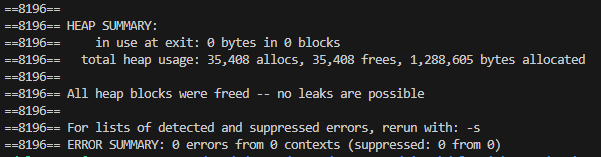
\includegraphics[width=0.98\textwidth]{./imgs/ValgrindOutput.PNG}}
    \caption{Valgrind Output (running command "valgrind ./main")}
    \label{fig:figure5-1}
\end{figure}

\noindent
In conclusion, this assignment was a great learning experience for me. This is my first time diving deep with C++ and so far, I'm having a great time. I struggled a little bit in the beginning, and also struggled during the implementation of Merge Sort and Quick Sort, but I got through it. With this assignment I also learned how to create a Makefile and also how to use Valgrind. The Makefile took a lot of my time because I tried to make it compatible with Windows and Linux. I had to read a lot of documentation and look up a ton of videos to find out how the file works and how to implement it specifically for my program. Valgrind was a very useful tool for me to use because it checks if memory leaks occur. One of the problems about C++ I was worried about was it doesn't automatically do garbage collection. However, with the help of Valgrind, I got my program from having more than 100,000 bytes of leakage down to 0. I can't wait to do more with C++ and algorithms as a whole. This is a ton of fun.

\end{document}
